% failuredetection.tex
\documentclass[dareport.tex]{subfiles}
\begin{document}
% Content here
\section{Failure Detection}

Initially, Naive approach is used to implement heartbeat failure detector in Strike Server. Each server will try to establish a short TCP connection to all peer severs for heartbeat interval X. Each server maintains a data structure of AliveMap<String, Integer>\footnote{ConcurrentHashMap in Java, with key (String) and value (Integer) } to store error factor for all known servers. i.e. \verb|{"sever1":0, "server2":3, "server3":1, "server4":2}| when we assume there are 4 servers in total. We will keep that assumption in the following discussion for simplicity. When \verb|server 1| fails to establish short TCP connection with \verb|server 2|, \verb|server 1| will modify its local AliveMap to increase the error factor of \verb|server 2| by 1. When the error factor of a particular server reaches Y, that server is considered as crashed. (Parameter X and Y can be set in configuration file) A server detecting any failed server will broadcast a message to all other servers to inform them deleting the failed server. This can be a problem in a partially connected network, a detected "fail server" will be remove from server list from all other servers since no consensus on deleting failure server is met. The consensus improvements will be discussed in consensus session.

Failure detection using Naive approach may works fine in a group of a few servers, however it is not effective when servers scale to a large number. For $N$ servers, there will be $O(N^{2})$ TCP connections among the servers for every heartbeat interval. This will lead to message explosion\cite{failuredetector}. A good failure detector in large scale distributed system must prevent flooding or overloading the network with failure detection related messages whereas the current heartbeat failure detector does not. Alternative approaches is needed.

To address this problem, we used gossip-type protocol to implement distributed algorithms in the chat system. In the article "Failure Detectors for Large-Scale Distributed Systems"\cite{failuredetector}, it introduces a basic gossiping protocol. Each host in the network maintains a failure detector maintaining a list with entries for all known hosts. These Each entry stores heartbeat counter for that particular host. A failure detection module will increase its own heartbeat counter, then pick another failure detection module randomly and send its list. Any failure detector module receiving this message will merge its local list by adopting the maximum heartbeat counter for each known host. If the heartbeat counter for host A  maintained by host B is not increased after some timeout, host A will be suspected by host B. 

However, the heartbeat counter will increase infinitely in the gossip list by using this approach and this is not desirable since the messages containing heartbeat counter list is passing between hosts. On the other hand, in our cases, Stike Servers may not get started exactly at the same time, so servers started slightly later will get suspected more easily. Bias in failure detection exists. Therefore, we decide to do other way around. Instead of increment own heartbeat count and merging gossip list by taking the maximum, heartbeat count for all remote servers is increased and the gossip list is merged by taking minimum. This approach is shown in data structure updates in GEMS\cite{gems}. For example, after Strike system running for a while and all server runs properly, the gossip list maintained by \verb|server 1| looks like \verb|{"sever1":0, "server2":1, "server3":0, "server4":2}| other than large heartbeat counters. we used that as a baseline of implementing gossip algorithm on our chat system. 

\subsection{Gossip Algorithm}
These are the steps of gossip algorithms and how it works in Strike System.

\begin{enumerate}[leftmargin=*]
\item Firstly, each server will run a failure detection module when it is started. We used Quartz Job Scheduling\footnote{http://www.quartz-scheduler.org/} to run this module as a job since Strike is developed in Java. There are three parameters needs to be configured for this job: "alive.interval" which represents gossip interval T in seconds, "alive.error.factor" F. 

\item Each server maintains a concurrent hashmap heartbeatCountList<String, Integer> to store heartbeat counts for all known servers and a concurrent hashmap suspectList<String, Integer> to store the current suspects(1 = suspected, 0 = not suspected).

\verb|heartbeatCountList = {"sever1":0, "server2":2, "server3":8, "server4":2}|
\verb|suspectList = {"sever1":0, "server2":0, "server3":1, "server4":0}|

For simplicity and easy understanding, "gossip list" connotes "HeartbeatCountList" in the following paragraphs.

\item For every T seconds, each failure detection module will reset its own heartbeat counter to 0 and increase the heartbeat counters of all remote servers. Then it picks another failure detection module randomly (another server) and send its gossip list using "gossip protocol" in Strike. (Shown in Figure: Gossip Module - Sending Gossip Message) The gossip message is in this format:
\verb|{"type":"gossip","serverid":"server1","heartbeatcountlist":{"server1":0,"server2":1,"server3":1,"server4":2}}|

\begin{figure}[h]
\label{fig:Gossip Module - Sending Gossip Message}
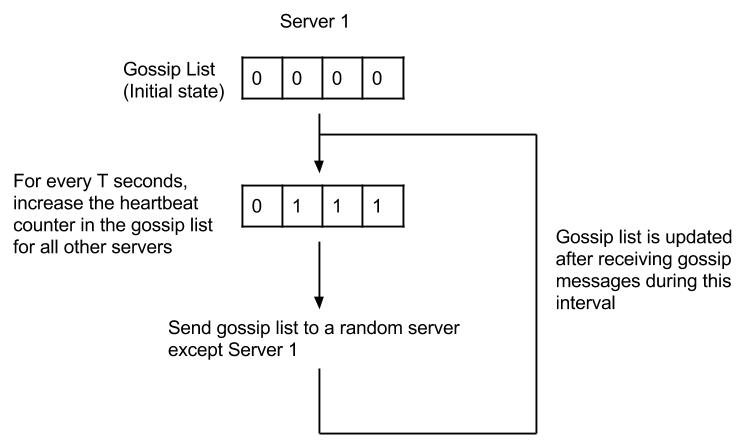
\includegraphics[scale=0.6]{gossip_send.jpg}
\caption{Gossip Module - Sending Gossip Message}
\centering
\end{figure}

\item Any server receiving gossip message will merge its local gossip list by adopting the maximum heartbeat counter for each known server. (Shown in Figure: Gossip Module - Receiving Gossip Message and Updating Gossip List)

\begin{figure}[h]
\label{fig:Gossip Module - Receiving Gossip Message and Updating Gossip List}
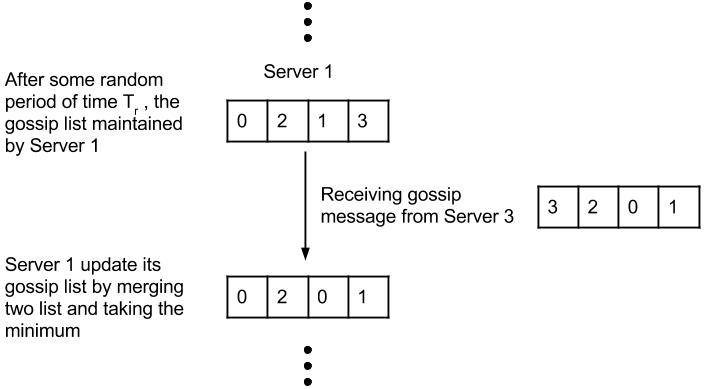
\includegraphics[scale=0.6]{gossip_receive.jpg}
\caption{Gossip Module - Receiving Gossip Message and Updating Gossip List}
\centering
\end{figure}


\item At any point of time, if the difference bewteen local heartbeat counter and the heartbeat counter of a remote server is greater than the error factor F, that particular remote server is suspected by the local server. For example, if the gossip list of \verb|server 1| is \verb|{"server1":0,"server2":5,"server3":1,"server4":2}| when error factor F = 5, \verb|server 1| suspects \verb|server 2| has crashed. And suspectList in Server 1 is updataed:

\verb|{"server1":0,"server2":1,"server3":0,"server4":0}|

\end{enumerate}

This algorithm differs from heartbeat failure detector such that instead of asking all other peers "Are you alive", each server now only select a random peer to gossip and share its view of the global state to that server. Eventually, all the correct servers will have agreements on the global state of Strike system. For example, if \verb|server 2| is crashed, the heartbeat counter of \verb|server 2| maintained by the failure detector module of all the other servers will be high because no server receives messages from \verb|server 2| and only \verb|server 2| can reset its own heartbeat counter. Gossip-type protocol solves the problem of message explosion as the number of TCP connections/messages among servers during gossip interval T is only N for N servers.


\end{document}